\chapter{Approach \& Implementation}
\label{ch:Approach}

\section{First approach: simple encoder}
\label{MyModel}
Our first plan to solve the Candidate Generation task was to approach it as a translation problem between two embedding spaces, i.e. from the mention embedding space to the knowledge graph embedding space. 
While building the system we tried to keep the architecture as simple as possible.

\begin{figure}[h]
\centering
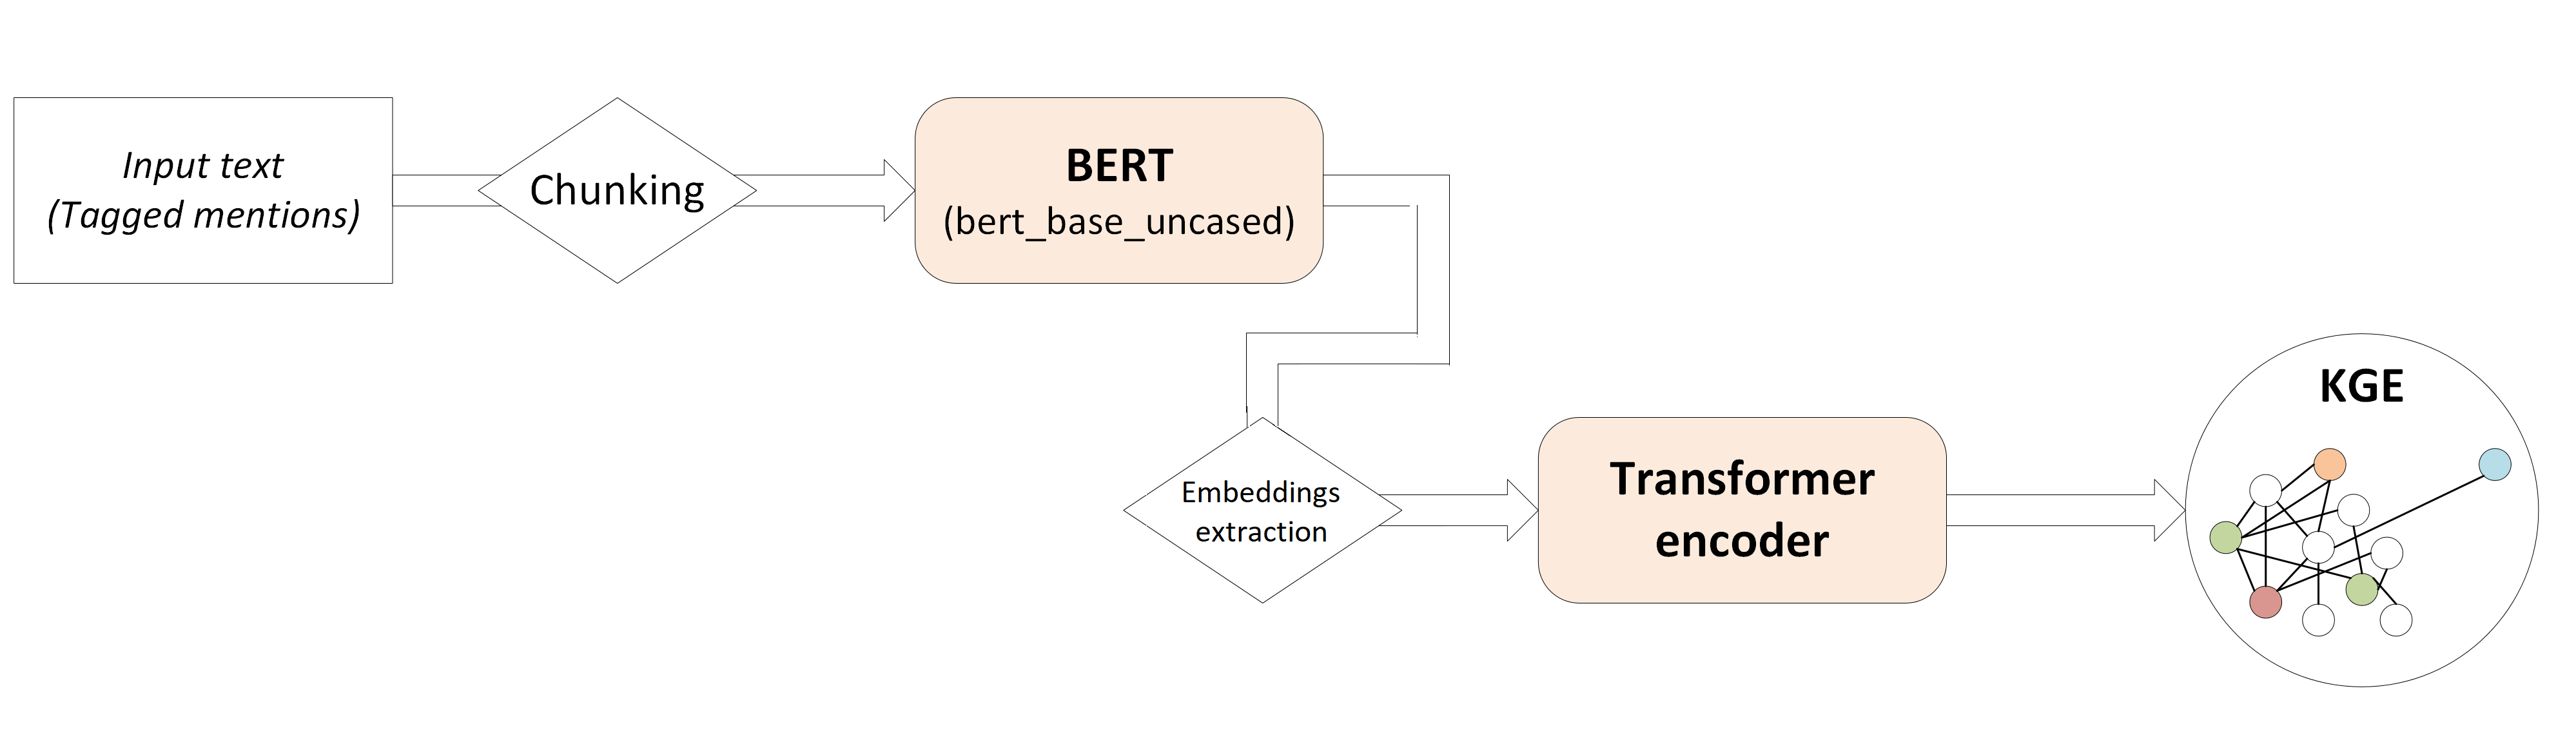
\includegraphics[width=16cm]{figures/MyImplementation.png}
\caption{The architecture of the system}
\label{My implementation}
\end{figure}

\subsection{Model's components}
As we can see in Figure\ref{My implementation}, two transformer encoders were used in the whole process. After preprocessing the input text (i.e. tagging, chunking) it is passed to a pre-trained BERT model, this first multi-layer encoder is used to generate the embeddings for the text. From the text embeddings, we then extract the mention embeddings. The latter vectors are given as input to the second encoder responsible for translating these embeddings to the knowledge graph embedding space. In section \ref{impl} we will go into more detail about the different states the input goes through.

\subsubsection{Mention encoder}
The architecture of this model was presented in \ref{transformer}. The particular model we use \textit{bert-base-uncased} consists of 12 layers, has a hidden size of 768, 12 self-attention heads, and 110M trainable parameters \cite{BERT}.\newline
This model takes, text as input. The input is of the following format \textit{[CLS]} text \textit{[SEP]}. 
From the output of this model, we extract the embeddings that will represent the mentions. Two methods were adopted for the extraction purpose. We will describe them in detail in section \ref{impl}.\newline

\subsubsection{Translator encoder}
This encoder has the same architecture as the previous one, however, the parameters are configurable so that we could test it in multiple ways and compare the performance of the different configurations.\newline
This encoder computes out of mentions embeddings a vector in the embedding space of the entities. This is the part of the system that will be trained and tested so that the returned vector is as close as possible to the embeddings of the target entity. The metrics we use to quantify the closeness of the prediction are described in \ref{training}\newline
Its input is the vectors of size 768\footnote{To achieve we have to pass the vector under the inputs\_embeds parameter of the forward method https://huggingface.co/docs/transformers/model\_doc/bert\#transformers.BertModel}. We chose this size so to keep the model simple and not to have to implement any modification to an already finished component, i.e. the mention encoder.\newline

\subsection{Implementation}
\label{impl}

In this section, we will describe thoroughly the different states the input goes through and how the final results are computed.\newline

\subsubsection{Pre-processing}
The preprocessing step aims to extract from the dataset the mention-entity pairs with which the model will be trained and then tested. To achieve this goal we first extract the lines containing the whole text. Given the spans for each mention's surface form, we surrounded the words forming the mention with the tags \textit{[m]} and \textit{[/m]} respectively representing the beginning and the end of the word/phrase. These steps were all accomplished with reliance on regular expressions. e.g. \textit{West Indian all-rounder [m] Phil Simmons [/m] took four for 38 on Friday}.\newline
Simultaneously we saved the URL of the entities to which the mentions refer to, in a dictionary in the same order they were encountered in the text.\newline
After tagging the mentions, the extracted texts are converted to tokens with the help of the BERT tokenizer, we then divide them into chunks. These chunks are composed of 256 token ids. The chunks that do not contain the appropriate number of tokens (256) are padded.\newline

As a final step before training, we load the entity embeddings in an index HNSW-graph \ref{HNSWG}
For the implementation of this data structure, we used the Faiss library \cite{FAISS}. We constructed the index with the following parameters:
\begin{itemize}
\item{\textit{M}=64, the number of neighbors used in the graph.}
\item{\textit{efSearch}=64}
\item{\textit{efConstruction}=64}
\end{itemize}
We chose these parameters in a way such that the search time and construction time are both kept short.

\subsubsection{Mentions embeddings}
\label{MenEmb}
To get the mentions embeddings we used two methods;

\begin{itemize}
\item{In the first method, we save the ids of the wordpieces that make up the mention surface form. We do this by first detecting all the mention spans in the chunk of text, with the help of the tags \textit{[m]} and \textit{[/m]}.\newline
We pass the text chunk ids to the BERT model, which returns an embedding matrix, which we will call $T_{13,256,768}$. We permute the dimension of the embedding to obtain $T_{256, 13, 768}$.\newline
Now for each token, we have 13 vectors of size 768 that represent its embedding at the different layers of the model.\newline
For a given mention $m$ in a text chunk, which is composed of \textit{k} wordpieces and starting at index \textit{s}, we compute the embedding as follows\footnote{This method was inspired from https://mccormickml.com/2019/05/14/BERT-word-embeddings-tutorial/}\footnote{In both equations \ref{embeddings} and \ref{embeddingsWithContext} the $\sum$ symbol denotes a pointwise addition of the vectors}}:
\begin{equation}
\label{embeddings}
embedding(m) = \dfrac{1}{k}\sum_{j=s}^{s+k} \dfrac{1}{4}\sum_{d=9}^{13}T_{j, d}
\end{equation}

\item{In the second method, we adopted the same approach but inspired by \cite{Wu2020}, instead of just combining the embeddings of the wordpieces that made the surface form, we further considered the context. We did this by including the embeddings of the 32 wordpieces that preceded and succeeded the start and the end tag  \textit{[m]} and \textit{[/m]} respectively.\newline
If the preceding or succeeding context does not contain 32 tokens (mention is at the start or end of the text) we use padding so that all the inputs have the same length. We chose the length to be equal to 78 because the longest mention span was 14 tokens, which with the 64 context tokens results in a sequence of 78 tokens\newline
Similar to the first method the embeddings are then computed as follows:
\begin{equation}
\label{embeddingsWithContext}
embedding(m) = \dfrac{1}{78}\sum_{j=s-32}^{s+k+32} \dfrac{1}{4}\sum_{d=9}^{13}T_{j, d}
\end{equation}
}
\end{itemize}

\subsubsection{Entities embeddings}
As for the entities we relied on pre-compiled embeddings for the knowledge graph \footnote{https://hobbitdata.informatik.uni-leipzig.de/KGE/PBG/DBpedia-2021-03/}. In the method used to generate these vectors, a distance-based scoring function is used (section \ref{kgeBK}). Entities are represented through coordinates 100-dimensional vectors in a Euclidean space and the relation between the different elements is represented by a translation vector.(Example: We consider the triple (\textit{head(h)}, \textit{predicate(p)}, \textit{tail(t)}), in this case vec(\textit{h}) + vec(\textit{l}) $\approx$ vec(\textit{t}). This embedding method was presented in \cite{TransE}.

\subsubsection{Training}
\label{training}
Before the training phase, we computed the embeddings for the mentions as we paired them with their respective golden entities. Afterward, we saved the data in a "tsv" file where the first element in each row is an ID for the text and the chunk of text respectively followed by the DBpedia link, then the mention, and finally the embedding of the mention.\newline During the training phase, we passed batches of 8, 768-dimensional vectors to the second encoder, which returned 100-dimensional vectors (equal to the dimensionality of the vectors into which the entities were encoded).
We tested two loss functions for this model; \newline

\textbf{First approach} was to set the negative log-likelihood as the training objective. We chose this function as other works with similar approaches that achieved high results relied on it as well (\cite{Wu2020}, \cite{logeswaran2019zero}). This technique although usually used for classification tasks, can also be adapted for the training of candidate generation models. In this case, we use neighboring vectors of the predicted vector as negative classes \cite{Sevgili2020}. The targets are then labeled by 1 if they correspond to the correct entity and by 0 otherwise.
The Binary Cross Entropy Loss with logits is then used to compute the loss of the model's prediction. This function is defined as follows \footnote{https://pytorch.org/docs/stable/generated/torch.nn.BCEWithLogitsLoss.html};

\begin{equation}
\label{BCE}
l(x, y) = L = {\{l_{1} \cdots l_{N}\}}^{\top}, l_{n} = -w_{n} [y_{n} \cdot \log\theta(x_{n}) + (1-y_{n}) \cdot \log(1-\theta(x_{n}))]
\end{equation} 

\textit{BCEWithLogitsLoss}: in Eq:\ref{BCE} the function $\theta$ represents the sigmoid function, which can be described as $\theta(x) = \dfrac{1}{1-e^{-x}}$, $w_{n}$ represents the weight of the n-th prediction, $x_{n}$ the model's prediction score, which in our case is represented by the dot product, and $y_{n}$ denotes the desired output. To compute the loss for each of the model's predictions, we set the reduction parameter to "mean", which implies we average the sum of all the l functions: \newline
\begin{equation}
\label{BCESum}
loss =  -\dfrac{1}{N}\sum_{i=0}^N l(x_{i}, y_{i})
\end{equation} 

A negative sign is added because the terms contained in the log functions are between 0 and 1 and so the sum will have a negative sign.\newline

Let us consider the example of the golden entity where $y_{n} = 1$ since it is the desired entity to be predicted. In this case the term $(1-y_{n}) \cdot \log(1-\theta(x_{n}))$ will be cancelled and we will be left with $y_{n} \cdot \log\theta(x_{n})$. In this case, if our prediction is far from the ground truth $\log\theta(x_{n})$, which represents the loss value for this prediction, will result in a great value and the contrary is to be expected in the inverse case.\newline 
Thus with this function, we can determine which predictions are close to and which are far from the desired output.

\textbf{Second approach} is more intuitive in contrast to the first one. We simply compute a distance representation between the prediction of the model and the actual target. We achieved this by summing the euclidean and cosine distance,

\begin{equation}
\label{cos+mse}
l(x, y) = 1 - CosineSimilarity(x, y) + MSE(x, y)
\end{equation}

The cosine similarity function\footnote{https://pytorch.org/docs/stable/generated/torch.nn.CosineSimilarity.html} $$CosineSimilarity(x_{1}, x_{2}) = \dfrac{x_{1} \cdot x_{2}}{max(\|x_{1}\|_{2} \cdot \|x_{2}\|_{2}, \epsilon)}$$

and the MSE function or the Mean Squared Error is defined as follows\footnote{https://pytorch.org/docs/stable/generated/torch.nn.MSELoss.html}: 
\begin{equation}
MSE(x, y) = L = {\{l_{1} \cdots l_{N}\}}^{\top}, l_{n}= (x_{n} - y_{n})^{2}
\end{equation}

\subsubsection{Changes to the initial approach}
The above-mentioned approaches could only predict the most frequent entities in the training dataset. So, under the assumption that the poor performance (Details of the tests and results can be found in the following Chapter \ref{ch:Evaluation}) is due to a lack of sufficient data, we replaced the second transformer encoder with a pre-trained BERT-model.\newline

We kept all the different steps of the pre-processing and the computation of the prediction the same and tested the model with the new component under the same conditions.\newline
%__________________________________________________________________________________________________________________________________________________________
%__________________________________________________________________________________________________________________________________________________________

\section{Second approach: BLINK model}
The performance of this model (Section \ref{MyModel}) was on par with its complexity. It performed poorly, especially with entities that were not seen, or only seen a few times during training. In more detail, we will go over the results of the evaluation of this first system in the subsequent chapter. In this section, we will discuss the second approach, that these results prompted. It consisted in trying to improve an already existing system, namely, BLINK from the work of \cite{Wu2020}.

\subsection{Model's components}
As briefly mentioned in chapter\ref{related Work}, and explained in \cite{Wu2020} the system is built out of two independent bi-encoder models, one for encoding mentions and their context and the other for encoding titles and descriptions of entities. The resulting vectors are then scored based on their dot product.\newline
In the usual implementation of the bi-encoder module, both encoders start with the same weights, and then during training, they update their weights independently from each other \cite{biencoder}.
Although the original model has also a crossencoder, in this work we will only use the bi-encoder as it is the only component needed for the task of candidate generation.\newline
In Figure\ref{BlinkMod} we show the example presented in \cite{Wu2020} with our addition to the model. We have left the structure of the Bi-Encoder model intact.
The latter consists of two pre-trained BERT models, i.e. \textit{bert-large-uncased}. Both of the encoders have the following configuration: 24-layers, 1024 hidden dimensions, 16 attention heads, and 336M parameters.\newline 
We have added a linear layer and a dropout layer to one of the encoders namely, the candidate encoder. This layer takes as input an embedding vector that we compiled by concatenating the knowledge graph embedding with the output of the candidate encoder, resulting in a vector of size (1024 + dimensions of the KGE). The output vector is then again brought down to the original size (1024) so that it can be mapped to the same dense space as the embeddings of the contexts.\newline


\begin{figure}[h]
\centering
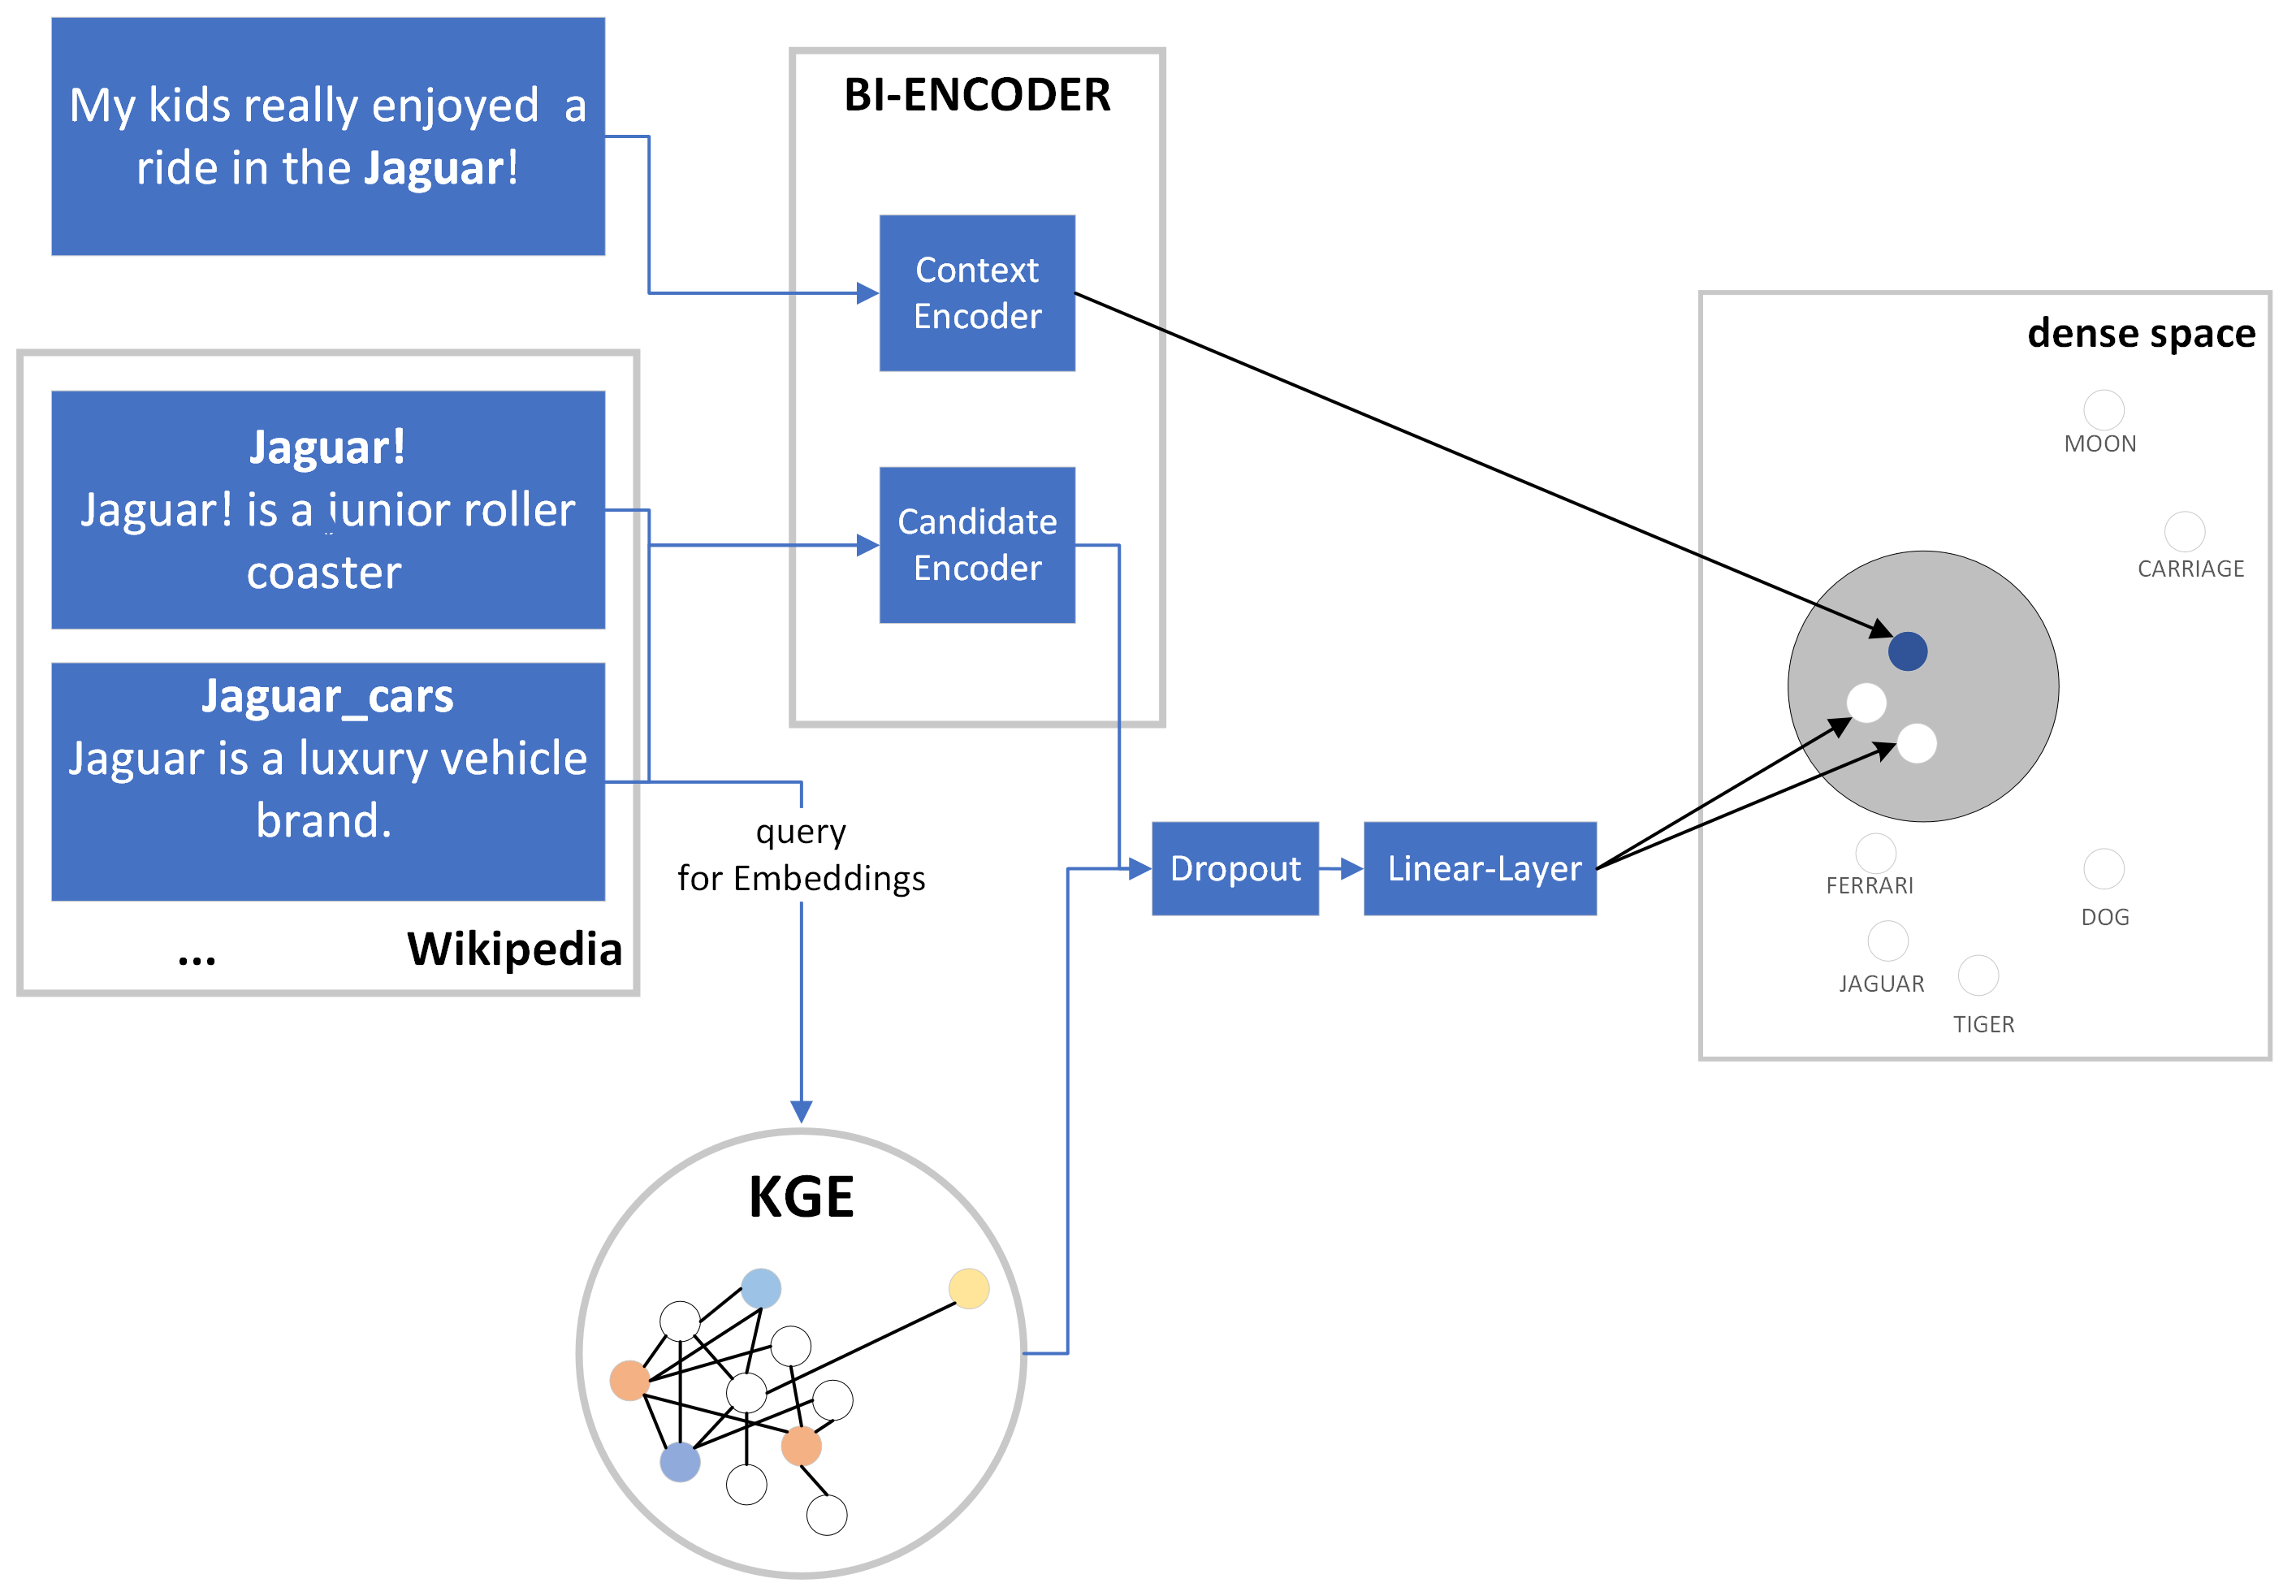
\includegraphics[width=12cm]{figures/NewBlinkVersion.png}
\caption{The architecture of the system}
\label{BlinkMod}
\end{figure}


\subsection{Implementation}
\subsubsection{Pre-processing}
We used the same datasets as in the first approach for training and evaluation. So we similarly extracted the mention-entity pairs as in the first approach, with the help of regular expressions.\newline
An additional pre-processing step that we implemented at this stage, was the extraction of labels and descriptions of entities from DBpedia dump files \footnote{https://databus.dbpedia.org/dbpedia/generic/}.\newline
We iterated through the entities present in the pre-computed knowledge graph embeddings, and for each URL we extracted the label and short abstract from the DBpedia dump files.\newline
Finally same as before (Section \ref{impl}) we constructed a HNSW-graph to hold the entities embeddings.\newline
\subsubsection{Mention embeddings}
Since the model was pre-trained we had to adopt similar techniques for the extraction of the embeddings for the mentions as presented in \cite{Wu2020}. Akin to the method described in Subsection \ref{MenEmb} (Second approach of mention embeddings) the mentions were embedded with a context window of 64 tokens, but there are two major differences. The first is that the contexts were submitted separately to the encoder as opposed to the whole text being encoded in one pass.\newline
The second difference lies in the embedding extraction method. The contexts were submitted under the following format [\textit{CLS}] text [\textit{start tag}] mention [\textit{end tag}] text [\textit{SEP}], and the embeddings were extracted from the \textit{CLS} token.\newline
The output of this first encoder was of size [batch-size x 1024]

\subsubsection{Entity embeddings}
The entities in \cite{Wu2020} were encoded based on their titles and descriptive text. So the embeddings were encryption of the textual context of the entity. Our idea was to expand the amount of information contained in these vectors by introducing the knowledge graph embeddings from DBpedia 2021\footnote{https://hobbitdata.informatik.uni-leipzig.de/KGE/PBG/DBpedia-2021-03/} as input along with the embedding of the textual description.\newline
Our goal was to enrich the entity embeddings with information about how the different entities relate to each other, to improve the mapping from one space to another, i.e. mentions embedding space, and entities embedding space.\newline
For entities that no short abstract was given, we just encoded the labels, and regarding entities that had no entry in the labels dump file, we used the last part of the URL and replaced the underscores "\_" with spaces, and removed any existent text between parentheses.\newline
Then a string was computed of the form [\textit{CLS}] labels [\textit{ENT}] short-abstract [\textit{SEP}] and passed through the entity encoder to obtain a contextual representation for the entity which is then saved with the URL and the pre-computed knowledge graph embeddings.\newline
And to obtain the final embeddings we concatenated the initial textual embedding with the knowledge graph embeddings of size [1024,] and [100,] respectively, and then passed the resulting vector through a linear layer to obtain the final representation vector of size [1024,].\newline

\subsubsection{Training}
After preprocessing the data, we loaded the model's weight's made available from \cite{Wu2020}, and then added the additional layers. 

During the training phase, we train both encoders of the bi-encoder simultaneously.\newline
Figure\ref{Training loop} represents the training pipeline, which includes the following steps;\newline
At first, we input the context of mentions as a vector of token ids through the context encoder of the biencoder. We have set all vectors to have the same size of 78. for the same reasons as in Section \ref{MenEmb}. Thus we obtained the embeddings for the mentions with their context ($m_{ctxt}$: size [1024,]).\newline
Using this output we query the index containing the initially textual computed embeddings for the entities to retrieve a set of k candidates. For each candidate in this set, we extract the TransE embeddings from a FAISS index that was previously generated and populated with the knowledge graph embeddings. We then concatenate both vectors and pass the newly 1124-dimensional vector through the added linear layer to compute the new representation. Following the same steps, we generate a vector for the golden entities. Thus we get newly generated embeddings, containing textual and contextual information for the set of k+1 candidate entities.\newline 
We then optimize the model using negative sampling. We label the k+1 candidates with 1 if they represent the correct entity and with 0 otherwise. Following this step, we compute the scores for the prediction and candidate set pairs. This is done by multiplying the matrices of the original size (\textit{batch-size} x \textit{embedding-size}) and (\textit{batch-size} x \textit{number-of-candidates} x \textit{embedding-size}) respectively. The latter matrices' sized are altered so we can perform the multiplication. We then pass the scores along with the labels to the loss function (Binary Cross Entropy with Logits) to obtain a scalar representation of the loss value.\newline
Finally, the weights of both models are updated.\newline

\begin{figure}[h]
\centering
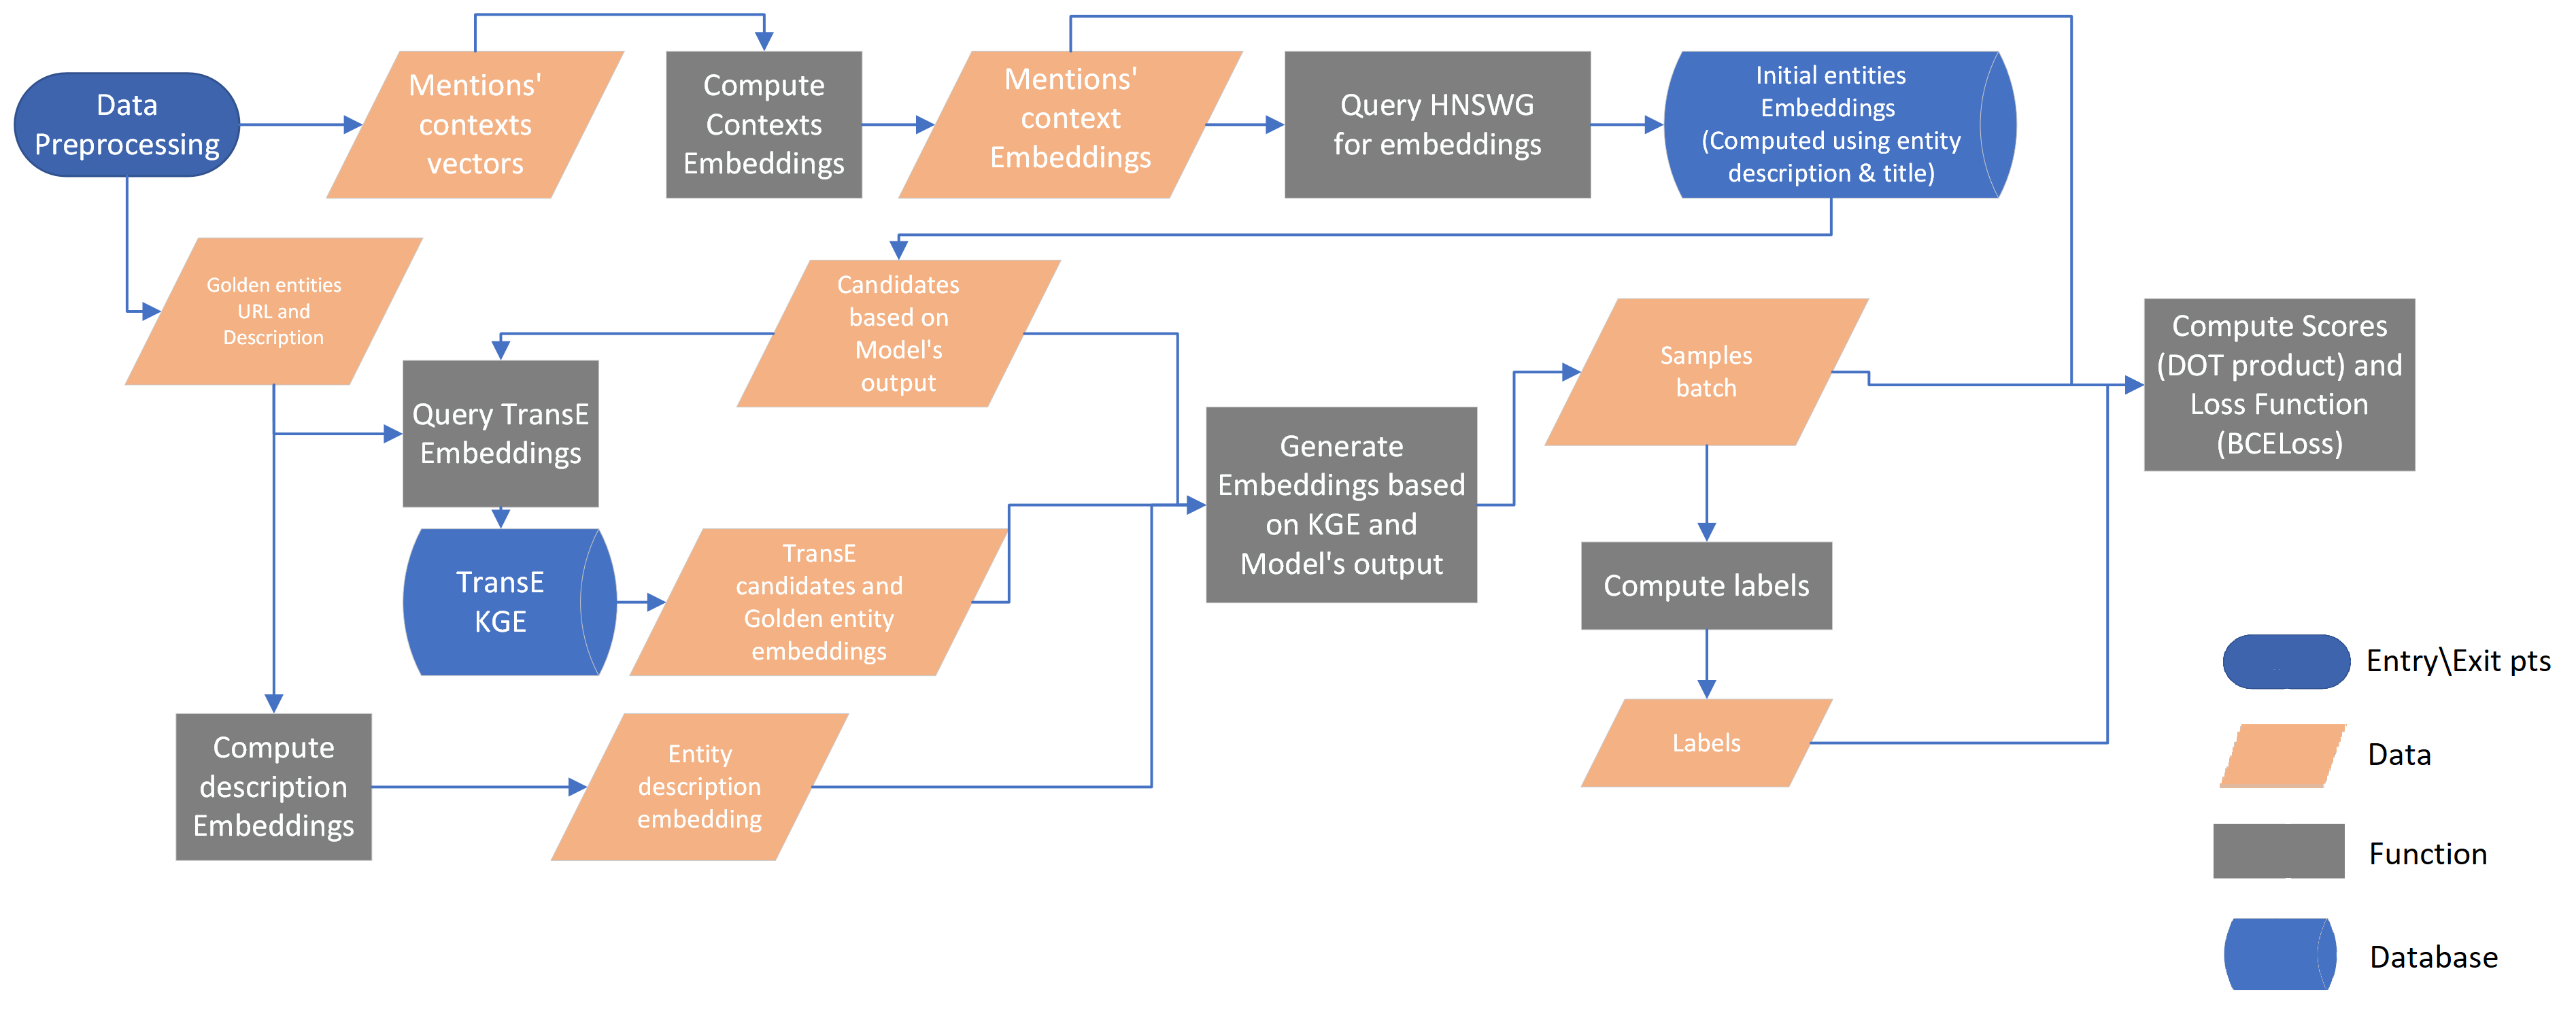
\includegraphics[width=17cm]{figures/TrainingFlowChart.png}
\caption{Training loop flow chart}
\label{Training loop}
\end{figure}

After fine-tuning the pre-trained model's weights, we use the newly obtained model to recompute the knowledge graph embeddings. And we then test the new model on the recalling rate from the newly generated embeddings.

%With the context encoder, we compute first the embeddings of the mentions' context, a vector of size (1, 1024). This vector is then in turn used to query the HNSW graph for the closest neighbors, which returns a batch of embeddings of size (1025)\footnote{in this case since the last dimension is used to convert from the DOT to the L2 similarity space since the HNSW supports only euclidean distance.}. These retrieved vectors with their respective URLs and the golden entity's computed description embedding and its corresponding URL are then all passed to the added linear layer (batch size, 1024) which outputs the final embeddings encoding the textual and relational information of the entities. We compute the label vectors for these candidates (1 for positives and 0 for negatives). Then we compute the loss by passing the scores of each output with each of its candidates and the labels to the loss function. The loss function is the Binary Cross Entropy loss function which is defined by the equation \ref{}.